
\documentclass[sigconf]{acmart}

\usepackage{graphicx}
\usepackage{booktabs}
\usepackage{hyperref}
\usepackage{subcaption}
\usepackage{listings}
\usepackage{tikz}
\usetikzlibrary{shapes,arrows,positioning,fit,backgrounds}

\title{A Proxy Persona Tool For Web Viewing and Chat Interaction}

\author{Christopher B. Rauch}
\affiliation{%
  \institution{Drexel University}
  \city{Philadelphia}
  \state{PA}
  \country{USA}
}
\email{cr625@drexel.edu}

\author{Hyung Wook Choi}
\affiliation{%
  \institution{Drexel University}
  \city{Philadelphia}
  \state{PA}
  \country{USA}
}
\email{hc685@drexel.edu}

\author{Michael L. Nelson}
\affiliation{%
  \institution{Old Dominion University}
  \city{Norfolk}
  \state{VA}
  \country{USA}
}
\email{mln@cs.odu.edu}

\author{Alex H. Poole}
\affiliation{%
  \institution{Drexel University}
  \city{Philadelphia}
  \state{PA}
  \country{USA}
}
\email{ahp56@drexel.edu}

\author{Travis Reid}
\affiliation{%
  \institution{Old Dominion University}
  \city{Norfolk}
  \state{VA}
  \country{USA}
}
\email{treid003@odu.edu}

\author{Michele C. Weigle}
\affiliation{%
  \institution{Old Dominion University}
  \city{Norfolk}
  \state{VA}
  \country{USA}
}
\email{mweigle@cs.odu.edu}

\author{Mat Kelly}
\affiliation{%
  \institution{Drexel University}
  \city{Philadelphia}
  \state{PA}
  \country{USA}
}
\email{mkelly@drexel.edu}

\begin{abstract}
This demo presents an interactive proxy tool designed to capture, inspect, and preserve personalized online activity in real-time browsing sessions. The system offers researchers and archivists a method to analyze the behaviors and presence of ads and other dynamic content during web interactions. The tool can be extended to provide context to Large Language Models that leverages the personalization options available in the major models and also allows persona information to be passed as additional context.
\end{abstract}

\keywords{web archiving, advertisements, proxy server, personalization}

\begin{document}
\begin{teaserfigure}
  \centering
  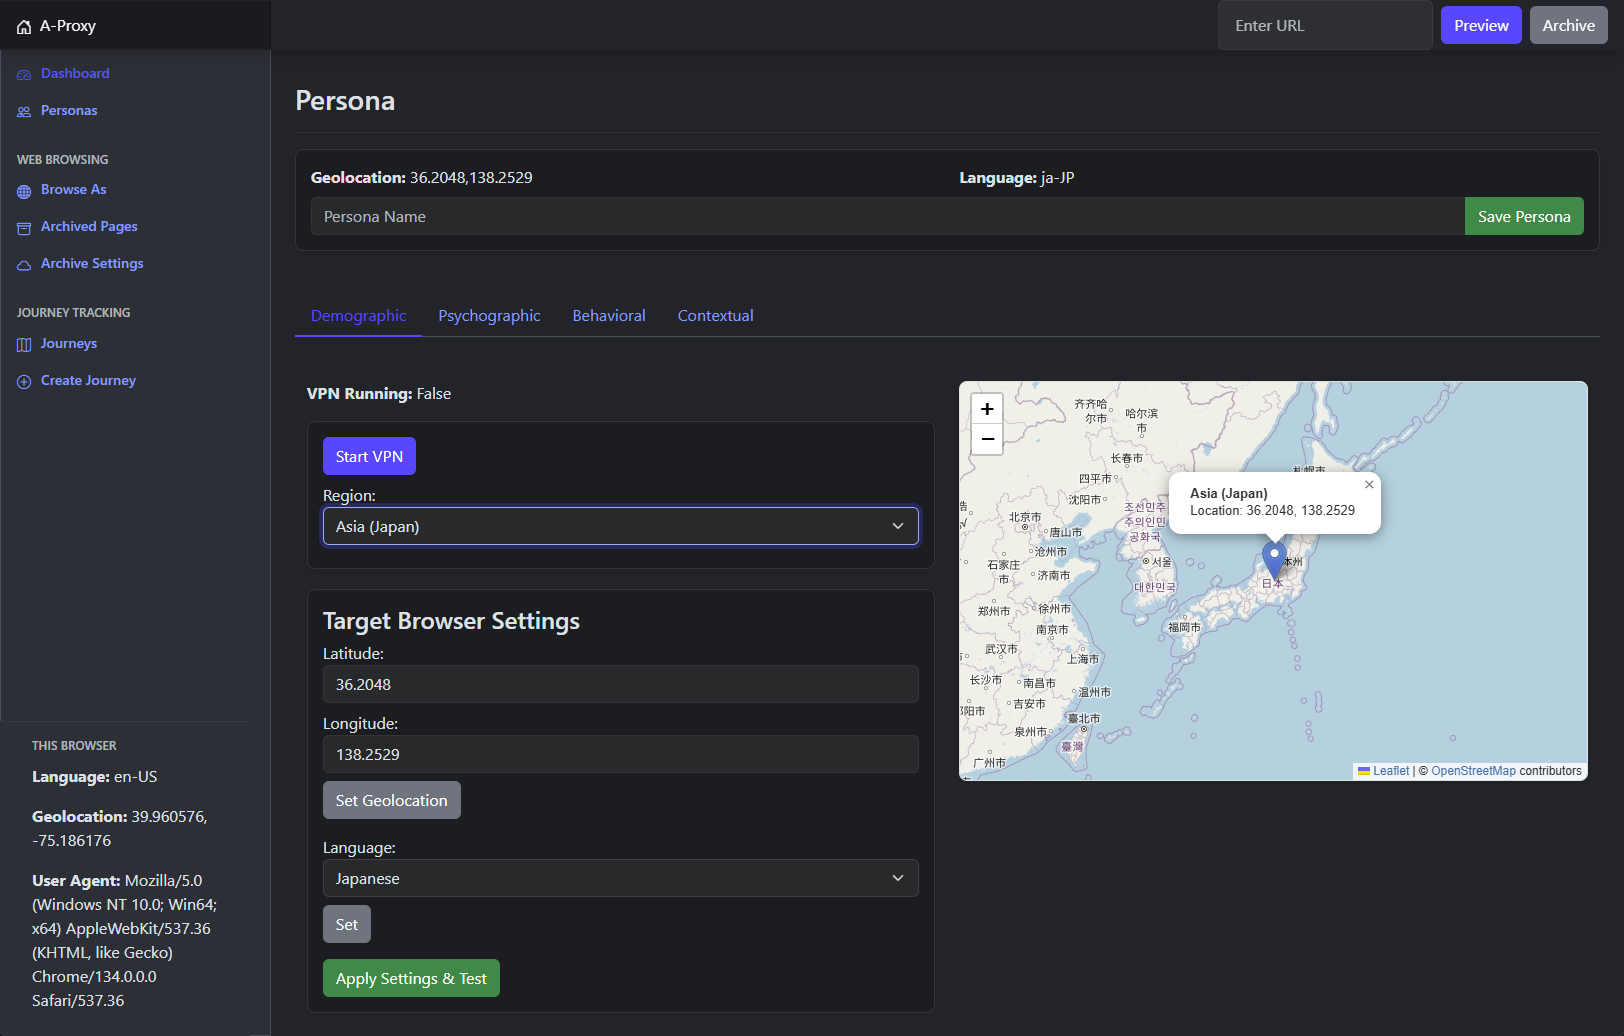
\includegraphics[width=\textwidth]{persona-teaser.png}
  \caption{Interface of the proxy system showing persona-level customization, including geolocation, language, and behavioral settings. The system enables fine-grained control over browser characteristics to simulate user experiences during web archiving or ad tracking.}
  \Description{Screenshot of A-Proxy interface showing persona settings, VPN toggle, and browser controls including geolocation and language.}
  \label{fig:persona}
\end{teaserfigure}
\maketitle


\section{Introduction}
Web advertisements are personalized according to marketing categories...

Advertisers gather data to customize content for each user, leveraging details such as demographics, behavior, and context to deliver highly personalized experiences. This data includes factors such as age, location, interests, and specific behavioral trends, including browsing habits and interaction styles. Adapting advertisements to user demographics improves relevance and engagement, leading to higher click-through rates and overall effectiveness \cite{de2015towards}. These practices allow businesses to refine their strategies by analyzing how different demographic groups respond to campaigns \cite{carrascosa2015always}. 

Kelly et al. (2013) \cite{kelly2013method} identified issues with personalized representations in web archiving and presented a prototype that extends GeoIP and browser environment. Specifically, they provided examples of how some websites display different contents, including news and weather information, depending on the user’s GeoIP or user-provided zip code. This shows how geolocation can impact the content presented to a user. Sowbhagya et al. (2022) \cite{hidri2024learning} explored how demographic information can be integrated with behavioral data to create more nuanced and accurate user profiles. Their research highlighted the importance of combining multiple data points to achieve more precise personalization, showing that demographic attributes often serve as crucial contextual markers that help interpret and predict user intentions and preferences. This multidimensional approach to user profiling allows for more refined targeting strategies and improved user experience customization.

Building on previous studies, similar strategies could be explored to improve the user experience in archives. Personalization techniques used in advertising, such as behavioral profiling and tracking, provide practical methods for capturing and representing individualized interactions with pages that are archived, but also for reproducing these interactions to simulate behavior. In this paper, we introduce A-Proxy, a tool that 



\section{System Overview}
A-Proxy is a comprehensive HTTP proxy system that intercepts and analyzes web traffic with a focus on personalization factors. The tool operates as a local proxy server that sits between the user's browser and the internet, capturing all HTTP/HTTPS requests and responses. By manipulating HTTP headers and browser settings, A-Proxy can simulate different user personas and geographic locations.

The system is designed with four key components: (1) a persona management system that maintains detailed user profiles including demographic, psychographic, behavioral, and contextual attributes; (2) a VPN integration layer that allows network traffic to appear from different global locations; (3) a browser customization module that modifies language preferences and geolocation settings; and (4) an archival system that captures and stores snapshots (mementos) of websites with associated metadata.

Users interact with A-Proxy through a web-based dashboard that provides real-time control over persona attributes and browsing parameters. The system can capture screenshots of rendered pages, record HTTP response headers, and organize browsing sessions into structured "journeys" for analysis. This comprehensive approach enables researchers and archivists to systematically examine how personalization affects web content delivery across different user contexts.

\section{System Architecture}
A-Proxy employs a modular architecture comprising five core components, as illustrated in Figure~\ref{fig:persona}.

The \textbf{Proxy Server} is built on Flask and serves as the central coordination point for all system operations. This component intercepts HTTP/HTTPS requests, modifies headers as needed, records traffic metrics, and provides the web interface for system control.

At the heart of the system is the \textbf{Persona Database}, an SQLite database that maintains comprehensive user personas with multiple attribute categories:
\begin{itemize}
    \item \textit{Demographic data}: Age, gender, location, language preferences, education, income
    \item \textit{Psychographic data}: Interests, values, attitudes, lifestyle, personality traits
    \item \textit{Behavioral data}: Browsing habits, purchase history, brand interactions, device usage
    \item \textit{Contextual data}: Time-based factors, device characteristics, environmental settings
\end{itemize}

The \textbf{VPN Integration Layer} connects to servers across multiple countries (including US, Brazil, Germany, Japan, and South Africa) to simulate different geographic origins. This component manages authentication, server selection, and connection state to ensure realistic geolocation simulation.

For browser-based customization, the \textbf{Browser Automation} module implements Selenium-based control to adjust language settings, override geolocation data, and capture screenshots of rendered pages. This enables the system to bypass client-side geolocation detection and present consistent persona characteristics.

Finally, the \textbf{Archive Management} component records website snapshots ("mementos") with associated metadata including timestamps, HTTP headers, and rendering information. The system maintains a historical record of how sites appear under different persona configurations.

The components interact through well-defined APIs, with the Flask application serving as the orchestration layer. Data flows from the user interface to the persona database, which configures the VPN and browser settings before requests are processed through the proxy server. Response data and screenshots are then stored in the archive system for future analysis.

\section{Demo Scenario}
Our demonstration will showcase A-Proxy's capabilities through three interactive scenarios that highlight its utility for different user groups, as illustrated in Figure~\ref{fig:demo-scenarios}.

\begin{figure}
\centering
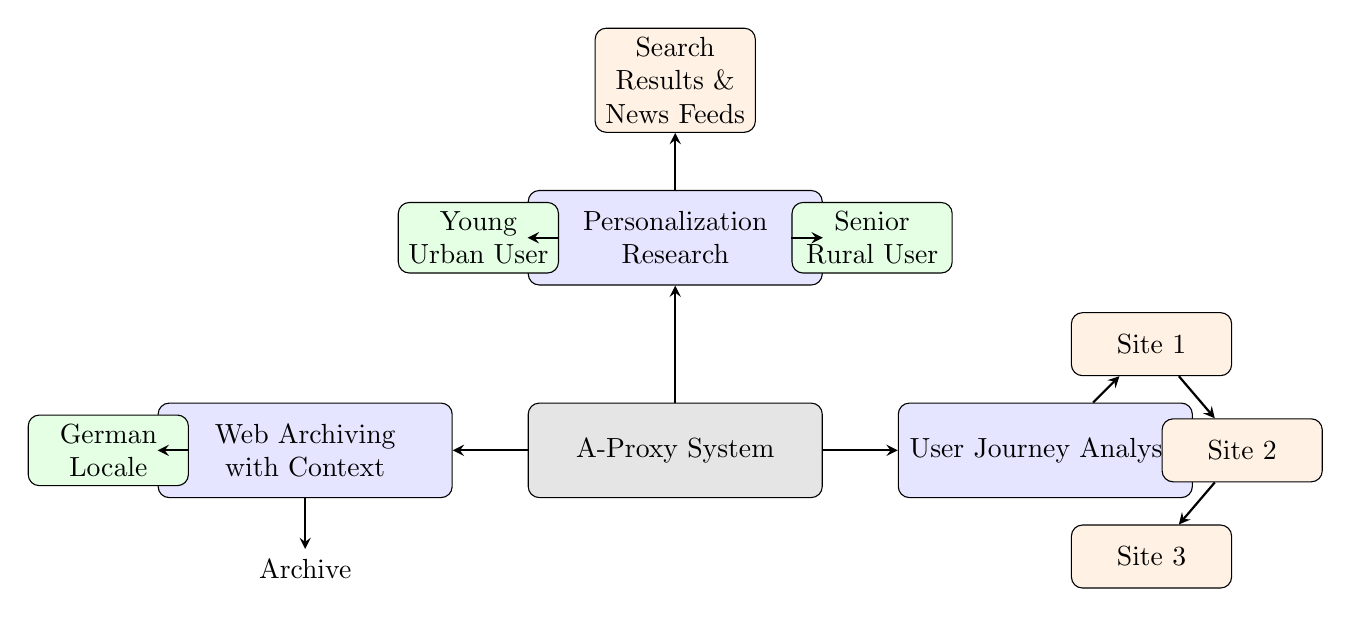
\begin{tikzpicture}[
    node distance=1.2cm,
    box/.style={rectangle, rounded corners, draw=black, text width=3.5cm, minimum height=1.2cm, align=center, fill=blue!10},
    arrow/.style={->, >=stealth, thick},
    persona/.style={rectangle, rounded corners, draw=black, text width=1.8cm, minimum height=0.8cm, align=center, fill=green!10},
    website/.style={rectangle, rounded corners, draw=black, text width=1.8cm, minimum height=0.8cm, align=center, fill=orange!10}
]
% Central A-Proxy system
\node[box, fill=gray!20] (proxy) {A-Proxy System};

% Scenario 1: Personalization Research
\node[box, above of=proxy, yshift=1.5cm] (scenario1) {Personalization Research};
\node[persona, left of=scenario1, xshift=-1.3cm] (persona1a) {Young Urban User};
\node[persona, right of=scenario1, xshift=1.3cm] (persona1b) {Senior Rural User};
\node[website, above of=scenario1, yshift=0.8cm] (website1) {Search Results \& News Feeds};

% Scenario 2: Web Archiving
\node[box, left of=proxy, xshift=-3.5cm] (scenario2) {Web Archiving with Context};
\node[persona, left of=scenario2, xshift=-1.3cm] (persona2) {German Locale};
\node[below of=scenario2, yshift=-0.3cm] (archive) {Archive};

% Scenario 3: User Journey
\node[box, right of=proxy, xshift=3.5cm] (scenario3) {User Journey Analysis};
\node[website, above right of=scenario3, xshift=0.5cm, yshift=0.5cm] (site1) {Site 1};
\node[website, right of=scenario3, xshift=1.3cm] (site2) {Site 2};
\node[website, below right of=scenario3, xshift=0.5cm, yshift=-0.5cm] (site3) {Site 3};

% Connections
\draw[arrow] (proxy) -- (scenario1);
\draw[arrow] (proxy) -- (scenario2);
\draw[arrow] (proxy) -- (scenario3);

\draw[arrow] (persona1a) -- (scenario1);
\draw[arrow] (persona1b) -- (scenario1);
\draw[arrow] (scenario1) -- (website1);

\draw[arrow] (persona2) -- (scenario2);
\draw[arrow] (scenario2) -- (archive);

\draw[arrow] (scenario3) -- (site1);
\draw[arrow] (site1) -- (site2);
\draw[arrow] (site2) -- (site3);

\end{tikzpicture}
\caption{A-Proxy demonstration scenarios: (1) Personalization Research compares website presentations across different user profiles; (2) Web Archiving with Context preserves personalized web views with their contextual metadata; and (3) User Journey Analysis tracks sequential interactions across multiple sites under consistent persona settings.}
\label{fig:demo-scenarios}
\end{figure}

In the \textbf{Personalization Research} scenario, we demonstrate how researchers can use A-Proxy to systematically investigate content personalization across platforms. Attendees will observe how search results, news feeds, and product recommendations change based on simulated user attributes. The demonstration will cycle through multiple demographic profiles (varying age, gender, location) while accessing the same websites, revealing algorithmic personalization patterns in real-time. This scenario showcases A-Proxy's value for critical algorithm studies and digital marketing research.

For digital preservationists, our \textbf{Web Archiving with Context} scenario demonstrates how A-Proxy creates contextualized web archives that capture personalization dimensions. Attendees will see how the tool archives not just page content but also the persona context that generated that view. We show how archived pages can be replayed with their original personalization context, addressing a significant gap in current web archiving methodologies. This scenario highlights A-Proxy's contribution to more comprehensive web preservation practices.

The \textbf{User Journey Analysis} scenario demonstrates A-Proxy's "journey" feature, which records sequences of web interactions under consistent persona settings. Attendees will see how marketing researchers, UX specialists, and scholars can use this functionality to analyze conversion pathways, content discovery patterns, and information-seeking behaviors. The tool visualizes these journeys and provides comparative analytics across different personas, enabling deeper understanding of user experience variations.

Throughout the demonstration, attendees can suggest websites to test with different persona configurations, allowing for interactive exploration of personalization mechanisms across the web.

\section{Implementation}
A-Proxy is implemented in Python, leveraging Flask for the web application framework and SQLite for data persistence. The system architecture follows a modular design pattern, with functionality separated into components that can be independently maintained and tested.

The core proxy functionality is implemented through a combination of Flask routes and middleware that intercept HTTP requests. Browser customization is handled via Selenium WebDriver, which provides programmatic control over Chrome instances. This enables the system to modify browser language settings and override geolocation data through the Chrome DevTools Protocol.

VPN integration leverages OpenVPN for secure connections to global server networks. The system dynamically manages VPN configurations and handles connection state through a dedicated service layer. Authentication and credential management are implemented with security best practices, including isolation of sensitive connection parameters.

The database schema includes normalized tables for personas (with related demographic, psychographic, behavioral, and contextual data), archived websites, mementos (snapshots), user journeys, and journey waypoints. This structure supports efficient querying while maintaining referential integrity through foreign key constraints.

For deployment flexibility, A-Proxy is containerized using Docker, with configuration handled through environment variables and volume mounts. This approach ensures consistency across development and production environments while simplifying dependency management.

The source code is available at: \url{https://github.com/savingads/a-proxy}

A demonstration video is accessible at: \url{[INSERT VIDEO LINK HERE]}

\section{Conclusion and Future Work}
A-Proxy provides researchers, archivists, and educators with a powerful tool for studying the increasingly personalized web. By combining proxy capabilities with persona management, geolocation simulation, and structured archiving, the system offers new methodological approaches for digital studies.

Future development will focus on several key areas. We plan to extend A-Proxy to support mobile traffic analysis through protocol-compatible proxy settings for iOS and Android devices, enabling research into the distinct personalization patterns of mobile web and app ecosystems. We will implement a real-time collaborative annotation system that allows team-based analysis of web content variations, supporting collaborative research projects where multiple analysts can tag, comment on, and categorize personalized content elements.

Advanced analytics capabilities will be developed to identify patterns in content variation across personas. This will include visualization components that highlight differences between persona views and quantify personalization intensity. We will also enhance interoperability with established web archiving platforms such as Archive-It and Webrecorder to support standardized preservation workflows, including implementing the WARC file format for broader compatibility with digital preservation systems.

A particularly promising direction is enhancing LLM integration. With Anthropic's recent open-sourcing of the Model Context Protocol (MCP), we can now develop more sophisticated methods for supplying contextual data to LLMs. Our next step is to add persona context data via API to LLM queries, allowing these models to better understand and interpret personalized content. This integration will leverage LLM capabilities to detect subtle content variations, characterize personalization strategies, and potentially simulate different user personas directly within the language model's reasoning process.

These enhancements will expand A-Proxy's utility beyond research and archiving to support educational use cases, regulatory compliance monitoring, and algorithmic transparency initiatives.

\bibliographystyle{ACM-Reference-Format}
\bibliography{software}

\end{document}
